%UCE-4: Testa environment

\begin{figure}
\centering
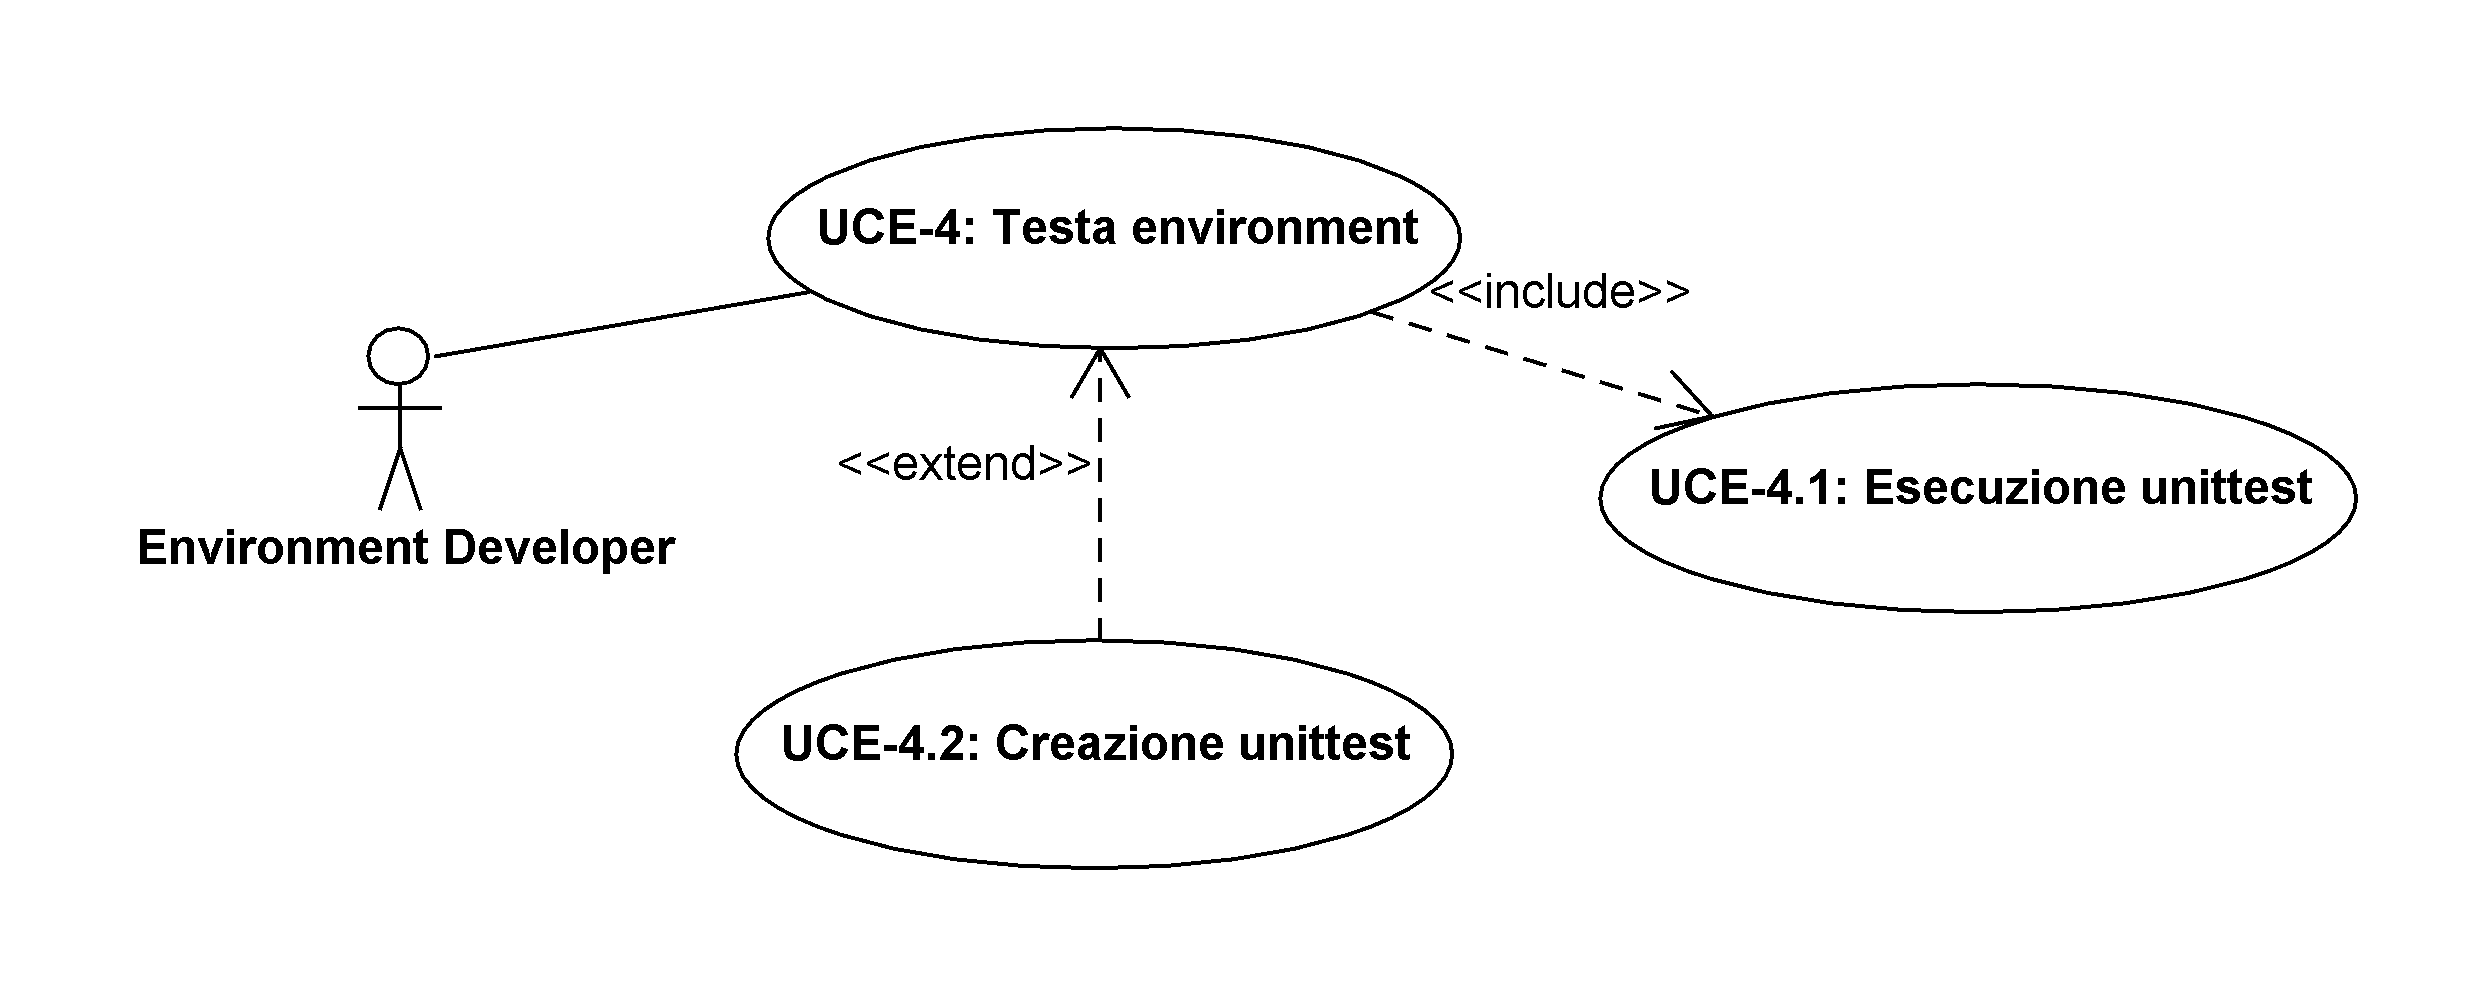
\includegraphics[width=1.1\textwidth]{Immagini/Capitolo2/UseCases/UCE-4.png}
\caption{Diagramma dei casi d'uso UCE-4}\label{fig:uc-uce-4}
\end{figure}

La descrizione comprende quella del caso d'uso \emph{UCE-4.1}.

\begin{itemize}
	\item \textbf{Attori:} ED
	\item \textbf{Scopo e descrizione:} l'ED deve essere in grado di verificare il funzionamento dell'environment utilizzando dei test d'unità. L'ED deve avere la possibilità di realizzare dei test d'unità per le funzionalità aggiunte
	\item \textbf{Pre-condizioni:} il software fornisce meccanismi per l'esecuzione di test d'unità in grado di verificare il comportamento dei componenti di sistema. Il software fornisce un framework per la definizione di nuovi test d'unità per le funzionalità introdotte
	\item \textbf{Post-condizioni:} l'ED ottiene dal software un riepilogo sul funzionamento delle componenti
	\item \textbf{Flusso principale degli eventi:}
		\begin{enumerate}
			\item l'ED avvia l'esecuzione dei test d'unità (\emph{UCE-4.1})
			\item l'ED ottiene un riepilogo dei risultati dei test
				\begin{itemize}
					\item il riepilogo indica eventuali test falliti
					\item il riepilogo indica il motivo del fallimento dei test
				\end{itemize}
		\end{enumerate}
\end{itemize}


\paragraph{UCE-4.1: Creazione unittest}

\begin{itemize}
	\item \textbf{Attori:} ED
	\item \textbf{Scopo e descrizione:} l'ED deve avere la possibilità di definire ed eseguire test d'unità in grado di verificare il corretto funzionamento delle caratteristiche aggiunte
	\item \textbf{Pre-condizioni:} il sistema è stato configurato correttamente. Il software offre meccanismi per l'integrazione di nuovi test d'unità a quelli forniti con il sistema
	\item \textbf{Post-condizioni:} un nuovo test d'unità è integrato con quelli forniti dal sistema
	\item \textbf{Flusso principale degli eventi:}
		\begin{enumerate}
			\item l'ED realizza un nuovo test d'unità
			\item l'ED registra il nuovo test d'unità insieme a quelli forniti dal software
		\end{enumerate}
\end{itemize}

